% Source for the figure of the distribution of the parallel sorts
% (sec. 25.6): a vector of 12 items in B = 3 blocks and k = 3 buckets,
% the counts of each block per bucket, their prefix sums in the order
% (bucket, block), and the buffer after the moves. Build: make figures (in
% ../build).
\documentclass[border=4pt]{standalone}
\usepackage[T1]{fontenc}
\usepackage{lmodern}
\usepackage{amsmath,amssymb}
\usepackage{tikz}
\usepackage{lamalunga}
% tikz-ads.tex: the TikZ styles shared by the figures of the memory of the
% manual, \input by each standalone figure: a cell of a vector (cell), the
% cell that an operation touches (touched), a free cell (free), a node of a
% linked structure (node), the labels of indices (index) and of variables
% (var), a pointer (ptr), and \cells and \indices to draw a row of cells.
\usetikzlibrary{arrows.meta,positioning,calc,fit,shapes.multipart}
\definecolor{adsTouched}{RGB}{214,196,236}
\definecolor{adsFree}{RGB}{236,236,236}
\tikzset{
  ads/.style={>={Stealth[length=2mm]},font=\small,
              every node/.append style={inner sep=0pt}},
  cell/.style={draw,minimum width=7mm,minimum height=7mm,
               font=\small\ttfamily,outer sep=0pt},
  touched/.style={cell,fill=adsTouched},
  free/.style={cell,fill=adsFree,text=black!45},
  node/.style={draw,rounded corners=1pt,minimum width=8mm,
               minimum height=6mm,font=\small\ttfamily},
  index/.style={font=\scriptsize\ttfamily,text=black!60},
  var/.style={font=\small\itshape},
  ptr/.style={->,thick}
}
% \cells{name}{x,y}{list}: a row of cells, the first at (x,y), named
% name-0, name-1, ...; each item is text/style, the style one of cell,
% touched and free (e.g., {a/cell,e/touched,/free})
\newcommand{\cells}[3]{%
  \foreach \v/\s [count=\i from 0] in {#3}
    \node[\s] (#1-\i) at ($(#2)+(\i*7mm,0)$) {\v};}
% \indices{name}{n}: the indices 0 .. n-1 under the cells of name
\newcommand{\indices}[2]{%
  \foreach \i in {0,...,\numexpr#2-1\relax}
    \node[index,below=1.2mm of #1-\i] {\i};}

\tikzset{b0/.style={cell},b1/.style={cell,fill=adsTouched},
         b2/.style={cell,fill=adsFree}}
\begin{document}
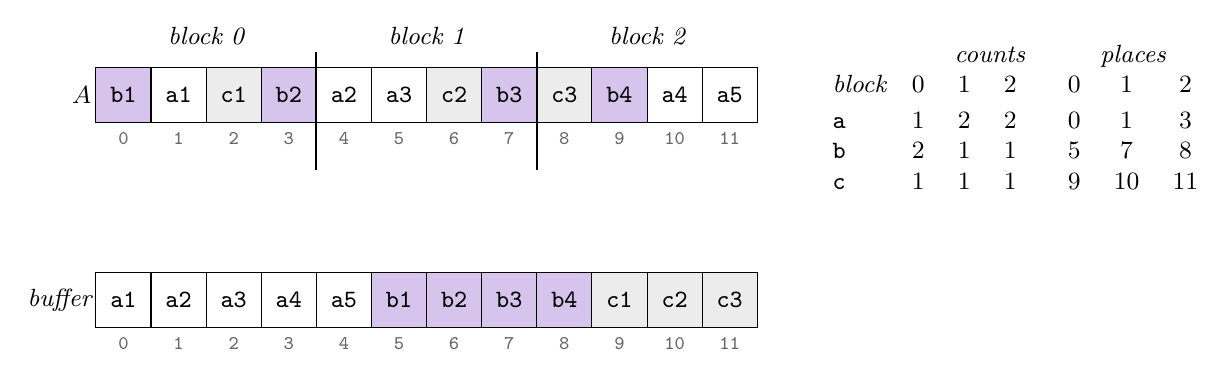
\begin{tikzpicture}[ads]
  \node[var,anchor=east] at (-4mm,0) {$A$};
  \cells{A}{0,0}{b1/b1,a1/b0,c1/b2,b2/b1,a2/b0,a3/b0,c2/b2,b3/b1,c3/b2,b4/b1,a4/b0,a5/b0}
  \indices{A}{12}
  \draw[thick] ($(A-3.north east)+(0,2mm)$) -- ($(A-3.south east)+(0,-6mm)$);
  \draw[thick] ($(A-7.north east)+(0,2mm)$) -- ($(A-7.south east)+(0,-6mm)$);
  \node[var] at ($(A-1.north east)+(0,4mm)$) {block 0};
  \node[var] at ($(A-5.north east)+(0,4mm)$) {block 1};
  \node[var] at ($(A-9.north east)+(0,4mm)$) {block 2};
  % the counts and the places
  \node[anchor=north west,font=\small] at (90mm,7mm) {%
    \begin{tabular}{@{}l@{\quad}ccc@{\qquad}ccc@{}}
      & \multicolumn{3}{c}{\itshape counts} &
        \multicolumn{3}{c}{\itshape places} \\
      \itshape block & 0 & 1 & 2 & 0 & 1 & 2 \\[2pt]
      \texttt{a} & 1 & 2 & 2 & 0 & 1 & 3 \\
      \texttt{b} & 2 & 1 & 1 & 5 & 7 & 8 \\
      \texttt{c} & 1 & 1 & 1 & 9 & 10 & 11
    \end{tabular}};
  \node[var,anchor=east] at (-4mm,-26mm) {buffer};
  \cells{Z}{0,-26mm}{a1/b0,a2/b0,a3/b0,a4/b0,a5/b0,b1/b1,b2/b1,b3/b1,b4/b1,c1/b2,c2/b2,c3/b2}
  \indices{Z}{12}
\end{tikzpicture}
\end{document}
